\section*{RESULTS}
\vspace{-4mm}
%%%%%%%%%%%%%%%%%%%%%%%%%%%%%%%%%%%%%%%%%%%%%%%%%%%%%%%%%%%%%%%%%%%%%%%%%%%%%%%%
%%%%  hp-FEM
The problem described above was solved using Hermes2D\footnote{http://hpfem.org/hermes2d/}, an open-source C++ library for adaptive $hp$-FEM solvers, currently under development at the University of Nevada at Reno.  We take advantage of the adaptive $hp$-FEM algorithms \cite{solin2010} from Hermes2D to solve the two physics on individual meshes.

%refine the mesh element or increase the polynomial degree

%%%%%%%%%%%%%%%%%%%%%%%%%%%%%%%%%%%%%%%%%%%%%%%%%%%%%%%%%%%%%%%%%%%%%%%%%%%%%%%%
%%%%  MMS
%\subsection*{Manufactured Solution}
The following choice for $\phi(\bx,t)$ and $T(\bx,t)$ was made
\begin{align}
  \left\{ \begin{array}{l}
      \phi(x,y,t) = C_\phi \left(1+\exp(r_\phi t)\right) \sin\left(\frac{\pi x}{L_X}\right) \sin\left(\frac{\pi y}{L_Y}\right) \frac{x}{L_X} \frac{y}{L_Y} \\
      T(x,y,t) = C_T \left(1+\tanh(r_T t)\right) \sin\left(\frac{\pi x}{L_X}\right) \sin\left(\frac{\pi y}{L_Y}\right)
  \end{array} \right.
\end{align}
and a script was written to perform the symbolic calculation of the forcing terms $Q_{\phi}(\bx,t)$ and $Q_T(\bx,t)$ so that the MMS can be used to verify the convergence to the exact solution when solving the nonlinear coupled multiphysics problem.

The solution $\phi(x,y)$ at time level $t=0.1 \mbox{sec}$ for adaptive $h$-FEM with quadratic quadrilateral elements ($p=2$) is shown in Fig. \ref{sol_temp}.  Since the exact solution is available, both the estimated error (comparing solution on coarse mesh with solution on finer mesh at each adaptivity step) and the exact error were computed.  The estimated error is slightly less than the exact one, but converges quickly to the exact error during adaptivity to become virtually identical (0.000186 \% for the estimated error versus 0.000187 \% in the solution for $\phi(x,y)$ in Fig. \ref{sol_temp}).
\begin{figure}
  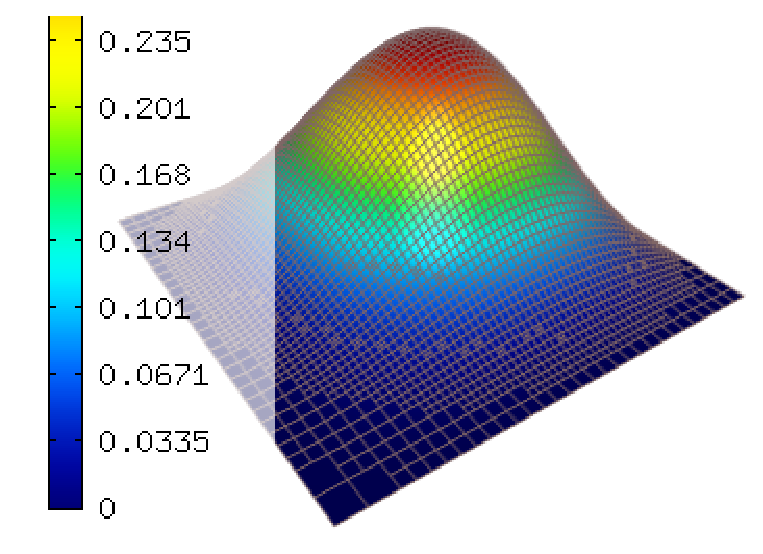
\includegraphics[width=0.5\textwidth]{figures/solution_T}
  \caption{Solution for $\phi(x,y)$ at time level $t=0.1 \mbox{sec}$ using adaptive $h$-FEM and $p=2$.  This contains 60353 DOFs and has a relative error 0.00019 \%.}
  \label{sol_temp}
\end{figure}

The problem was solved using both $h$-adaptivity with linear ($p=1$) as well as quadratic ($p=2$) quadrilateral elements and $hp$-adaptivity.  Fig. \ref{err_conv} shows the convergence rate for the temperature $T(x,y)$ at time level $t=0.1 \mbox{sec}$ in terms of the size of the number of degrees of freedom (DOFs).
\begin{figure}
  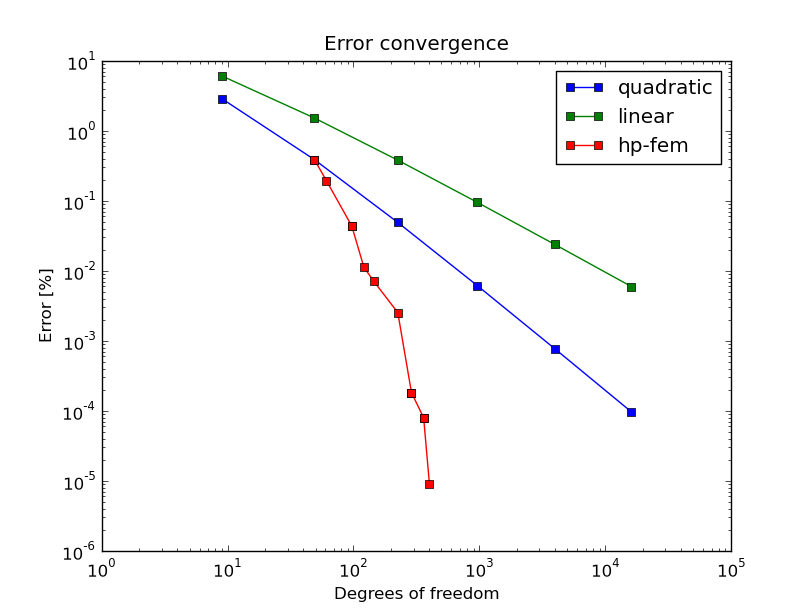
\includegraphics[width=0.5\textwidth]{figures/exact_err_conv}
  \caption{Convergence comparison of adaptive $hp$-FEM with adaptive $h$-FEM on linar ($p=1$) and quadratic ($p=2$) finite elements.  The error plotted is the exact relative error in norm $L_2$ for the temperature $T(x,y)$ at time level $t=0.1 \mbox{sec}$.}
  \label{err_conv}
\end{figure}

The error ploted is the relative error in $L_2$ norm, between the numerical results $T$ and the analytical solution $T_{exact}$.  It is computed using
\begin{align}
  e = \frac{ \|T-T_{exact}\|_{L_2} }{ \|T_{exact}\|_{L_2} }
\end{align}

As noted on that figure, the convergence graphs of adaptive $h$-FEM show the slopes in $-p/d$ (where $d$ is the dimension) on the log-log scale predicted by the theory, and adaptive $hp$-FEM does reach exponential convergence.
